% A4横・2分割の演習プリントテンプレート
\documentclass[paper=a4,landscape,twocolumn,fleqn]{jlreq}
\special{papersize=\the\paperwidth,\the\paperheight}
\setlength{\columnseprule}{0.4pt}
\pagestyle{empty}

\usepackage[margin=10truemm]{geometry}
\usepackage[dvipdfmx]{graphicx}
\usepackage{amsmath,amssymb}
\usepackage{tikz}
\usepackage{pgfplots}
\pgfplotsset{compat=1.18}
\usetikzlibrary{arrows.meta,calc,angles,quotes}

\ModifyHeading{section}{
  lines=1,
  before_space=8pt,
  after_space=0pt
}

\begin{document}

\section{計算問題}
次の式を計算せよ。
\begin{align*}
  1.\;& (x+3)^2 = \\
  2.\;& (2a-1)(a+4) = \\
  3.\;& \sqrt{72} =
\end{align*}

\section{図形問題（図を見て答える）}
次の図で，点 $A(1,2)$，$B(5,4)$ とする。\
\begin{minipage}{0.48\columnwidth}
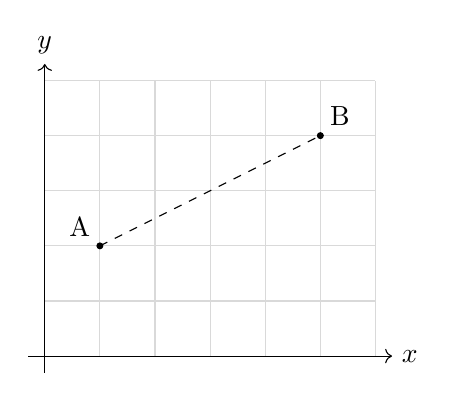
\begin{tikzpicture}[scale=0.7]
  \draw[gray!30] (0,0) grid (6,5);
  \draw[->] (-0.3,0) -- (6.3,0) node[right] {$x$};
  \draw[->] (0,-0.3) -- (0,5.3) node[above] {$y$};
  \filldraw (1,2) circle (1.5pt) node[above left] {A};
  \filldraw (5,4) circle (1.5pt) node[above right] {B};
  \draw[dashed] (1,2) -- (5,4);
\end{tikzpicture}
\end{minipage}
\begin{minipage}{0.48\columnwidth}
1. 線分 $AB$ の傾きは \underline{\hspace{2cm}} \\
2. 距離 $AB$ は \underline{\hspace{2cm}}
\end{minipage}

\section{三角比の穴埋め}
\begin{minipage}{0.45\columnwidth}
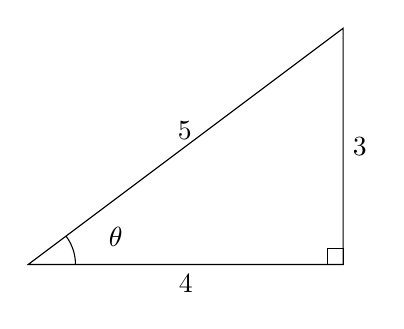
\begin{tikzpicture}[scale=1.0]
  \coordinate (A) at (0,0);
  \coordinate (B) at (4,0);
  \coordinate (C) at (4,3);
  \draw (A)--(B)--(C)--cycle;
  \draw (4,0) rectangle (3.8,0.2);
  \node[below] at (2,0) {4};
  \node[right] at (4,1.5) {3};
  \node[left] at (2.2,1.7) {5};
  \draw (0.6,0) arc[start angle=0,end angle=36.87,radius=0.6];
  \node[right] at (0.9,0.35) {$\theta$};
\end{tikzpicture}
\end{minipage}
\begin{minipage}{0.5\columnwidth}
$\sin\theta = \dfrac{\underline{\hspace{0.8cm}}}{\underline{\hspace{0.8cm}}} = \underline{\hspace{1.5cm}}$ \\
$\cos\theta = \dfrac{\underline{\hspace{0.8cm}}}{\underline{\hspace{0.8cm}}} = \underline{\hspace{1.5cm}}$ \\
$\tan\theta = \dfrac{\underline{\hspace{0.8cm}}}{\underline{\hspace{0.8cm}}} = \underline{\hspace{1.5cm}}$
\end{minipage}

\newpage
\section{関数グラフ読解}
下のグラフを見て答えよ。
\begin{center}
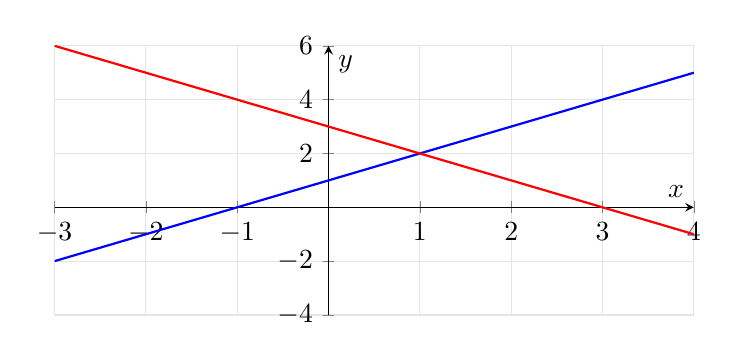
\begin{tikzpicture}
  \begin{axis}[
    width=0.8\columnwidth,
    height=5.0cm,
    axis lines=middle,
    xmin=-3,xmax=4,
    ymin=-4,ymax=6,
    xlabel={$x$},ylabel={$y$},
    grid=both,
    grid style={gray!20}
  ]
    \addplot[blue,thick,domain=-3:4]{x+1};
    \addplot[red,thick,domain=-3:4]{-x+3};
  \end{axis}
\end{tikzpicture}
\end{center}
1. 2直線の交点は \underline{\hspace{2.5cm}} \\
2. $x=2$ のとき，青い直線の $y$ 座標は \underline{\hspace{2cm}}

\end{document}
